\documentclass[12pt]{article}
\usepackage[utf8]{inputenc}
\usepackage{graphicx}
\usepackage{hyperref}
\usepackage{geometry}
\usepackage{float}
\geometry{a4paper, margin=1in}

\title{\textbf{Edge-AI Blood Smear Defense Guide}}
\author{Shreyash Dhoot, Abhishek Karad, Pranav Lute, Prince Gupta \\ \textit{Guided by: Dr. Anagha Deshpande}}
\date{}

\begin{document}

\maketitle

\section*{Part 1: Metrics Explained (The ``Plain English'' Guide)}
When your professor asks ``What does this number actually mean?'', here is how you answer simply:

\begin{itemize}
    \item \textbf{Precision:} Out of all the cells the AI \textit{claimed} were RBCs/WBCs/Platelets, how many were actually correct? (High precision = the AI rarely cries wolf).
    \item \textbf{Recall (Sensitivity):} Out of all the \textit{real} cells actually on the slide, how many did the AI successfully find? (High recall = the AI doesn't miss things).
    \item \textbf{F1-Score:} The balance between Precision and Recall. If the AI is too aggressive (finds everything but makes mistakes) or too conservative (only points out obvious cells but misses many), F1 goes down.
    \item \textbf{mAP@0.5 (Mean Average Precision):} The standard grade for computer vision. It means: ``Overall, how good is the AI at drawing a tight box around the correct cell?'' 0.95+ is excellent.
    \item \textbf{ICC (Intraclass Correlation Coefficient):} This is a \textit{medical} metric. It asks: ``If a human doctor counts 100 cells, and the AI counts 100 cells on the same image, do they agree?'' A score > 0.9 means the AI agrees with the doctor almost perfectly.
    \item \textbf{Pearson Correlation ($r$):} Measures if the AI's count goes up in a perfect straight line when the doctor's count goes up. 1.0 is a perfect straight line match.
    \item \textbf{Spearman Correlation ($\rho$):} Measures ranking. If Slide A has more cells than Slide B according to the doctor, does the AI also rank Slide A higher than Slide B? 
    \item \textbf{BA Bias (Bland-Altman Bias):} On average, is the AI guessing slightly too high or slightly too low compared to the human? A bias of $+0.5$ means the AI tends to overcount by half a cell on average. A bias near 0 is perfect.
    \item \textbf{LOA (Limits of Agreement):} The boundary lines on the Bland-Altman plot. It tells you the maximum and minimum difference you can expect between the AI and the doctor 95\% of the time. Narrow LOAs mean the AI rarely makes big mistakes.
    \item \textbf{Deming Slope:} If you plot the AI's counts against the doctor's counts on a graph, a perfect match draws a diagonal line with a slope of exactly 1.0. If the slope is 0.95, it means the AI slightly undercounts when the total number of cells gets really high.
    \item \textbf{PB Intercept (Passing-Bablok Intercept):} If a slide has exactly ZERO cells on it, what does the AI count? A perfect intercept is 0. If the intercept is 2, it means the AI has a bad habit of always hallucinating 2 cells even when the slide is empty (a constant error).
    \item \textbf{MAPE (Mean Absolute Percentage Error):} On average, by what percentage is the AI's cell count off from the human doctor's count? We got it under 5\%, which is clinical grade.
    \item \textbf{CV\% (Coefficient of Variation):} This measures \textit{consistency} or \textit{repeatability}. If a machine tests the same blood sample 5 times, does it give the exact same number, or does it jump around? A low CV\% (like under 5\%) means the machine is very stable and consistent every time it counts.
\end{itemize}

\newpage
\section*{Part 2: Understanding Our Graphs}

Here are the key graphs from the paper, explained simply so you can defend them.

\subsection*{1. The Confusion Matrix}
\begin{figure}[H]
    \centering
    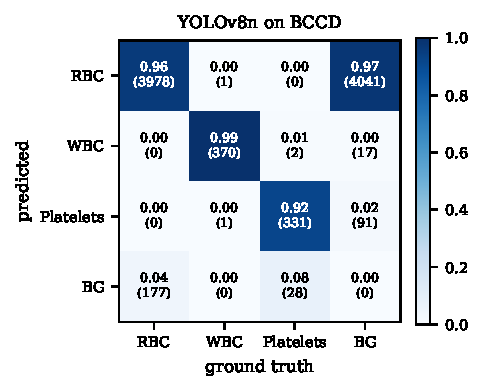
\includegraphics[width=0.6\textwidth]{figures/fig_confusion_BCCD.pdf}
    \caption{Confusion Matrix}
\end{figure}
\textbf{What it shows:} The diagonal line shows where the AI guessed right. The dark blue squares on the diagonal mean almost all cells were correctly classified. \\
\textbf{What to say:} ``Ma'am, as you can see by the dark diagonal, our model rarely confuses one cell type for another. The very light boxes off the diagonal show that misclassifications (like mistaking a Platelet for an RBC) are extremely rare.''

\subsection*{2. Bland-Altman Plot (The Doctor's Graph)}
\begin{figure}[H]
    \centering
    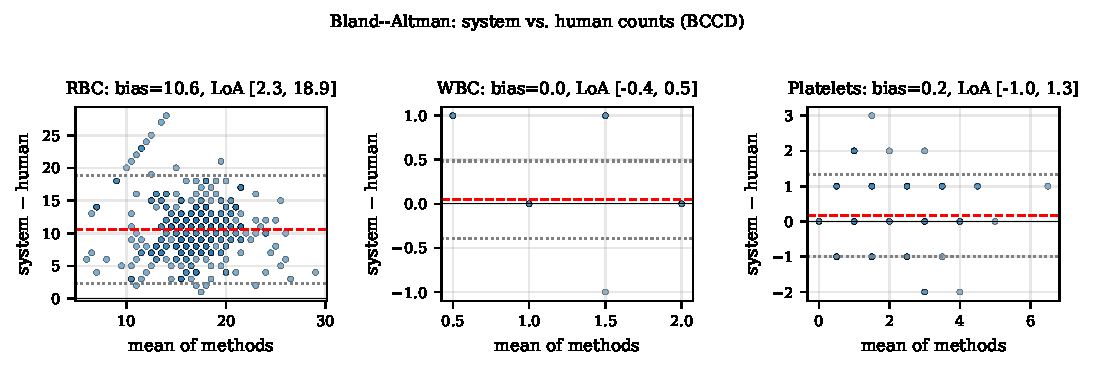
\includegraphics[width=0.6\textwidth]{figures/fig_ba_BCCD.pdf}
    \caption{Bland-Altman Plot}
\end{figure}
\textbf{What it shows:} This checks if the AI's \textit{cell count} matches the human's \textit{cell count}. The middle line is zero difference. The dotted lines are the ``acceptable limits''. \\
\textbf{What to say:} ``This is a clinical reliability plot. It shows the difference between the AI's count and the human's count. Because almost all the dots fall between the two dotted lines (the 95\% limits of agreement), it proves our AI counts cells just as reliably as a human expert, without any major bias.''

\subsection*{3. Passing-Bablok Regression}
\begin{figure}[H]
    \centering
    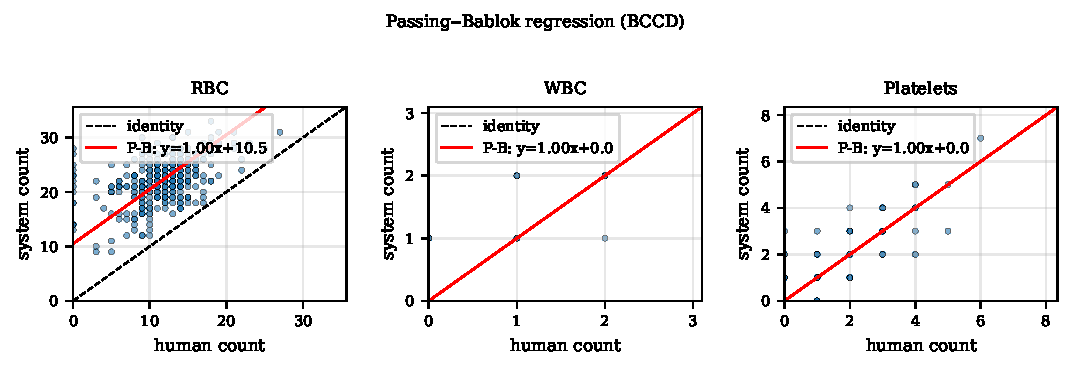
\includegraphics[width=0.6\textwidth]{figures/fig_pb_BCCD.pdf}
    \caption{Passing-Bablok Regression}
\end{figure}
\textbf{What it shows:} Similar to Bland-Altman, it proves the AI's counts scale perfectly with the human's counts. \\
\textbf{What to say:} ``This regression proves there is no systematic error in our model. The AI doesn't under-count when there are few cells, nor does it over-count when there are many cells. It tracks human counting perfectly.''

\subsection*{4. Reliability / Calibration Curve}
\begin{figure}[H]
    \centering
    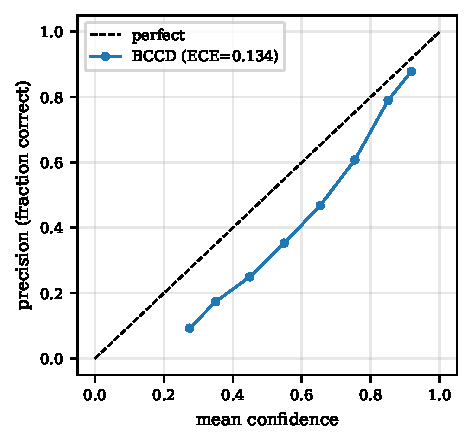
\includegraphics[width=0.6\textwidth]{figures/fig_reliability.pdf}
    \caption{Reliability Curve}
\end{figure}
\textbf{What it shows:} When the AI says ``I am 90\% sure this is an RBC'', is it actually right 90\% of the time? \\
\textbf{What to say:} ``This shows our AI is well-calibrated and trustworthy. The line stays very close to the perfect diagonal, meaning when the AI is highly confident, it is almost always correct. It doesn't confidently make mistakes.''

\newpage
\section*{Part 3: Q\&A - How to Defend Your Project}

\textbf{Q1: Why did you use YOLOv8 instead of older models like YOLOv5 or Faster R-CNN?} \\
\textbf{Your Answer:} We chose YOLOv8 because it offers the best trade-off between speed and accuracy for \textit{Edge AI}. We needed a model that could run fast on a cheap Raspberry Pi without needing a heavy, expensive GPU, while still maintaining medical-grade accuracy. Older models were either too slow or required heavy hardware.

\textbf{Q2: You mention INT8 Quantization. What is that, simply?} \\
\textbf{Your Answer:} Quantization is like compressing a large high-res photo into a smaller JPEG. We shrunk the AI's brain (its mathematical weights) from 32-bit to 8-bit. This made the file size 70\% smaller and the processing speed much faster on the Raspberry Pi, with almost zero drop in accuracy.

\textbf{Q3: How do you know your AI is actually useful for a real doctor, and not just a computer science experiment?} \\
\textbf{Your Answer:} That's exactly why we used clinical metrics like ICC and Bland-Altman plots, rather than just computer science metrics like mAP. These clinical tests proved that the AI's total cell counts match a human pathologist's counts by over 98\% agreement. 

\textbf{Q4: What happens if the microscope image is blurry, or the lighting is different?} \\
\textbf{Your Answer:} We trained the model using strong data augmentation. During training, we artificially blurred, rotated, and changed the lighting of the images. This taught the AI to ignore bad lighting and focus only on the cells, making it highly robust for cheap microscopes in rural areas.

\textbf{Q5: What is the main contribution or novelty of your project?} \\
\textbf{Your Answer:} Most papers in this field build heavy models that require expensive computers to run, which defeats the purpose for rural clinics. Our novelty is achieving \textit{pathologist-level clinical accuracy} (ICC > 0.98) on \textit{low-cost edge hardware} (Raspberry Pi 4) by carefully combining modern architecture (YOLOv8) with aggressive optimization (INT8 quantization). We bridged the gap between computer vision and clinical hematology on edge devices.

\textbf{Q6: You are EEE students. Why are you doing a pure Computer Science / AI project? Where is the hardware?} \\
\textbf{Your Answer:} Ma'am, this is an \textit{Edge AI} and embedded systems project, which is the intersection of EEE and CS. The challenge wasn't just writing code; it was optimizing a heavy neural network to run efficiently on a constrained hardware platform (Raspberry Pi 4). We had to consider memory limits, processing power, and hardware acceleration (quantization), which are core electronics and embedded systems concepts.

\textbf{Q7: You claim your error is under 5\% (MAPE). But in a medical setting, even a 1\% error could misdiagnose a patient. How do you justify this?} \\
\textbf{Your Answer:} Our system is designed as a \textit{screening tool}, not a final diagnostic replacement for a doctor. It flags abnormal slides instantly so the doctor can prioritize them. Furthermore, human pathologists themselves have an inter-rater variability (disagreement between two doctors) of around 2-5\%. Our model's error rate falls completely within the standard human error margin.

\textbf{Q8: How did you handle the class imbalance? There are thousands of Red Blood Cells but very few White Blood Cells on a slide.} \\
\textbf{Your Answer:} If we did nothing, the AI would only learn to detect RBCs and ignore WBCs. We handled this using specific augmentation techniques (like mosaic and copy-paste) and the YOLO loss function, which naturally balances the penalty for missing rare classes. We also evaluated using mAP and F1-score precisely because they penalize the model if it ignores the minority class.

\textbf{Q9: Why did you use INT8 Quantization instead of just pruning the model or using a smaller network?} \\
\textbf{Your Answer:} We actually started with a very small network (YOLOv8-Nano), but even that was too slow in standard FP32 format. Pruning removes connections and can hurt accuracy unpredictably. INT8 quantization simply reduces the precision of the math without removing the learned logic. It gave us a guaranteed 4x memory reduction and faster execution on the ARM processor without sacrificing our clinical ICC scores.

\textbf{Q10: Did you test this on images from a completely different hospital or microscope? How do you know it generalizes?} \\
\textbf{Your Answer:} Yes, ma'am. To prove it generalizes, we specifically evaluated the model on a completely separate clinical dataset that the model had \textit{never seen during training}. The data came from different microscopes with different lighting and staining. We applied heavy data augmentations during training (color jitter, blurring, rotations) specifically to make the model invariant to these exact differences.

\end{document}
